\chapter{Конструкторская часть}

В данном разделе разработаны схемы реализаций алгоритма расчета термовой частоты для всех термов из выборки документов.

\section{Требования к программному обеспечению}

К программе предъявлены ряд требований:

\begin{itemize}[label=---]
	\item иметь интерфейс для выбора действий;
	\item динамически выделять память под массив данных;
	\item работа с массивами и <<нативными>> потоками;
	\item замерять процессорное время работы реализаций алгоритмов.
\end{itemize}

\section{Разработка алгоритмов}

На рисунках \ref{fig:tf} -- \ref{fig:thread_work} приведены схемы однопоточной и многопоточной реализаций алгоритма расчета термовой частота для всех термов из выборки документов.
Вспомогательному потоку в числе аргументов в качестве структуры будут переданы:
\begin{itemize}
	\item start\_doc --- номер строки для начало работы, разбивающего цикла по вспомогательным потокам;
	\item end\_doc  --- номер строки для конца работы, разбивающего цикла по вспомогательным потокам;
	\item docs --- документы для обработки;  
	\item cltn --- данные полученные после обработки.
\end{itemize}
По первым двум из перечисленных аргументов будет определен объем работы, выполняемый конкретным вспомогательным потоком, то есть на интервале $[start\_doc, end\_doc]$.

\begin{figure}[h]
	\centering
	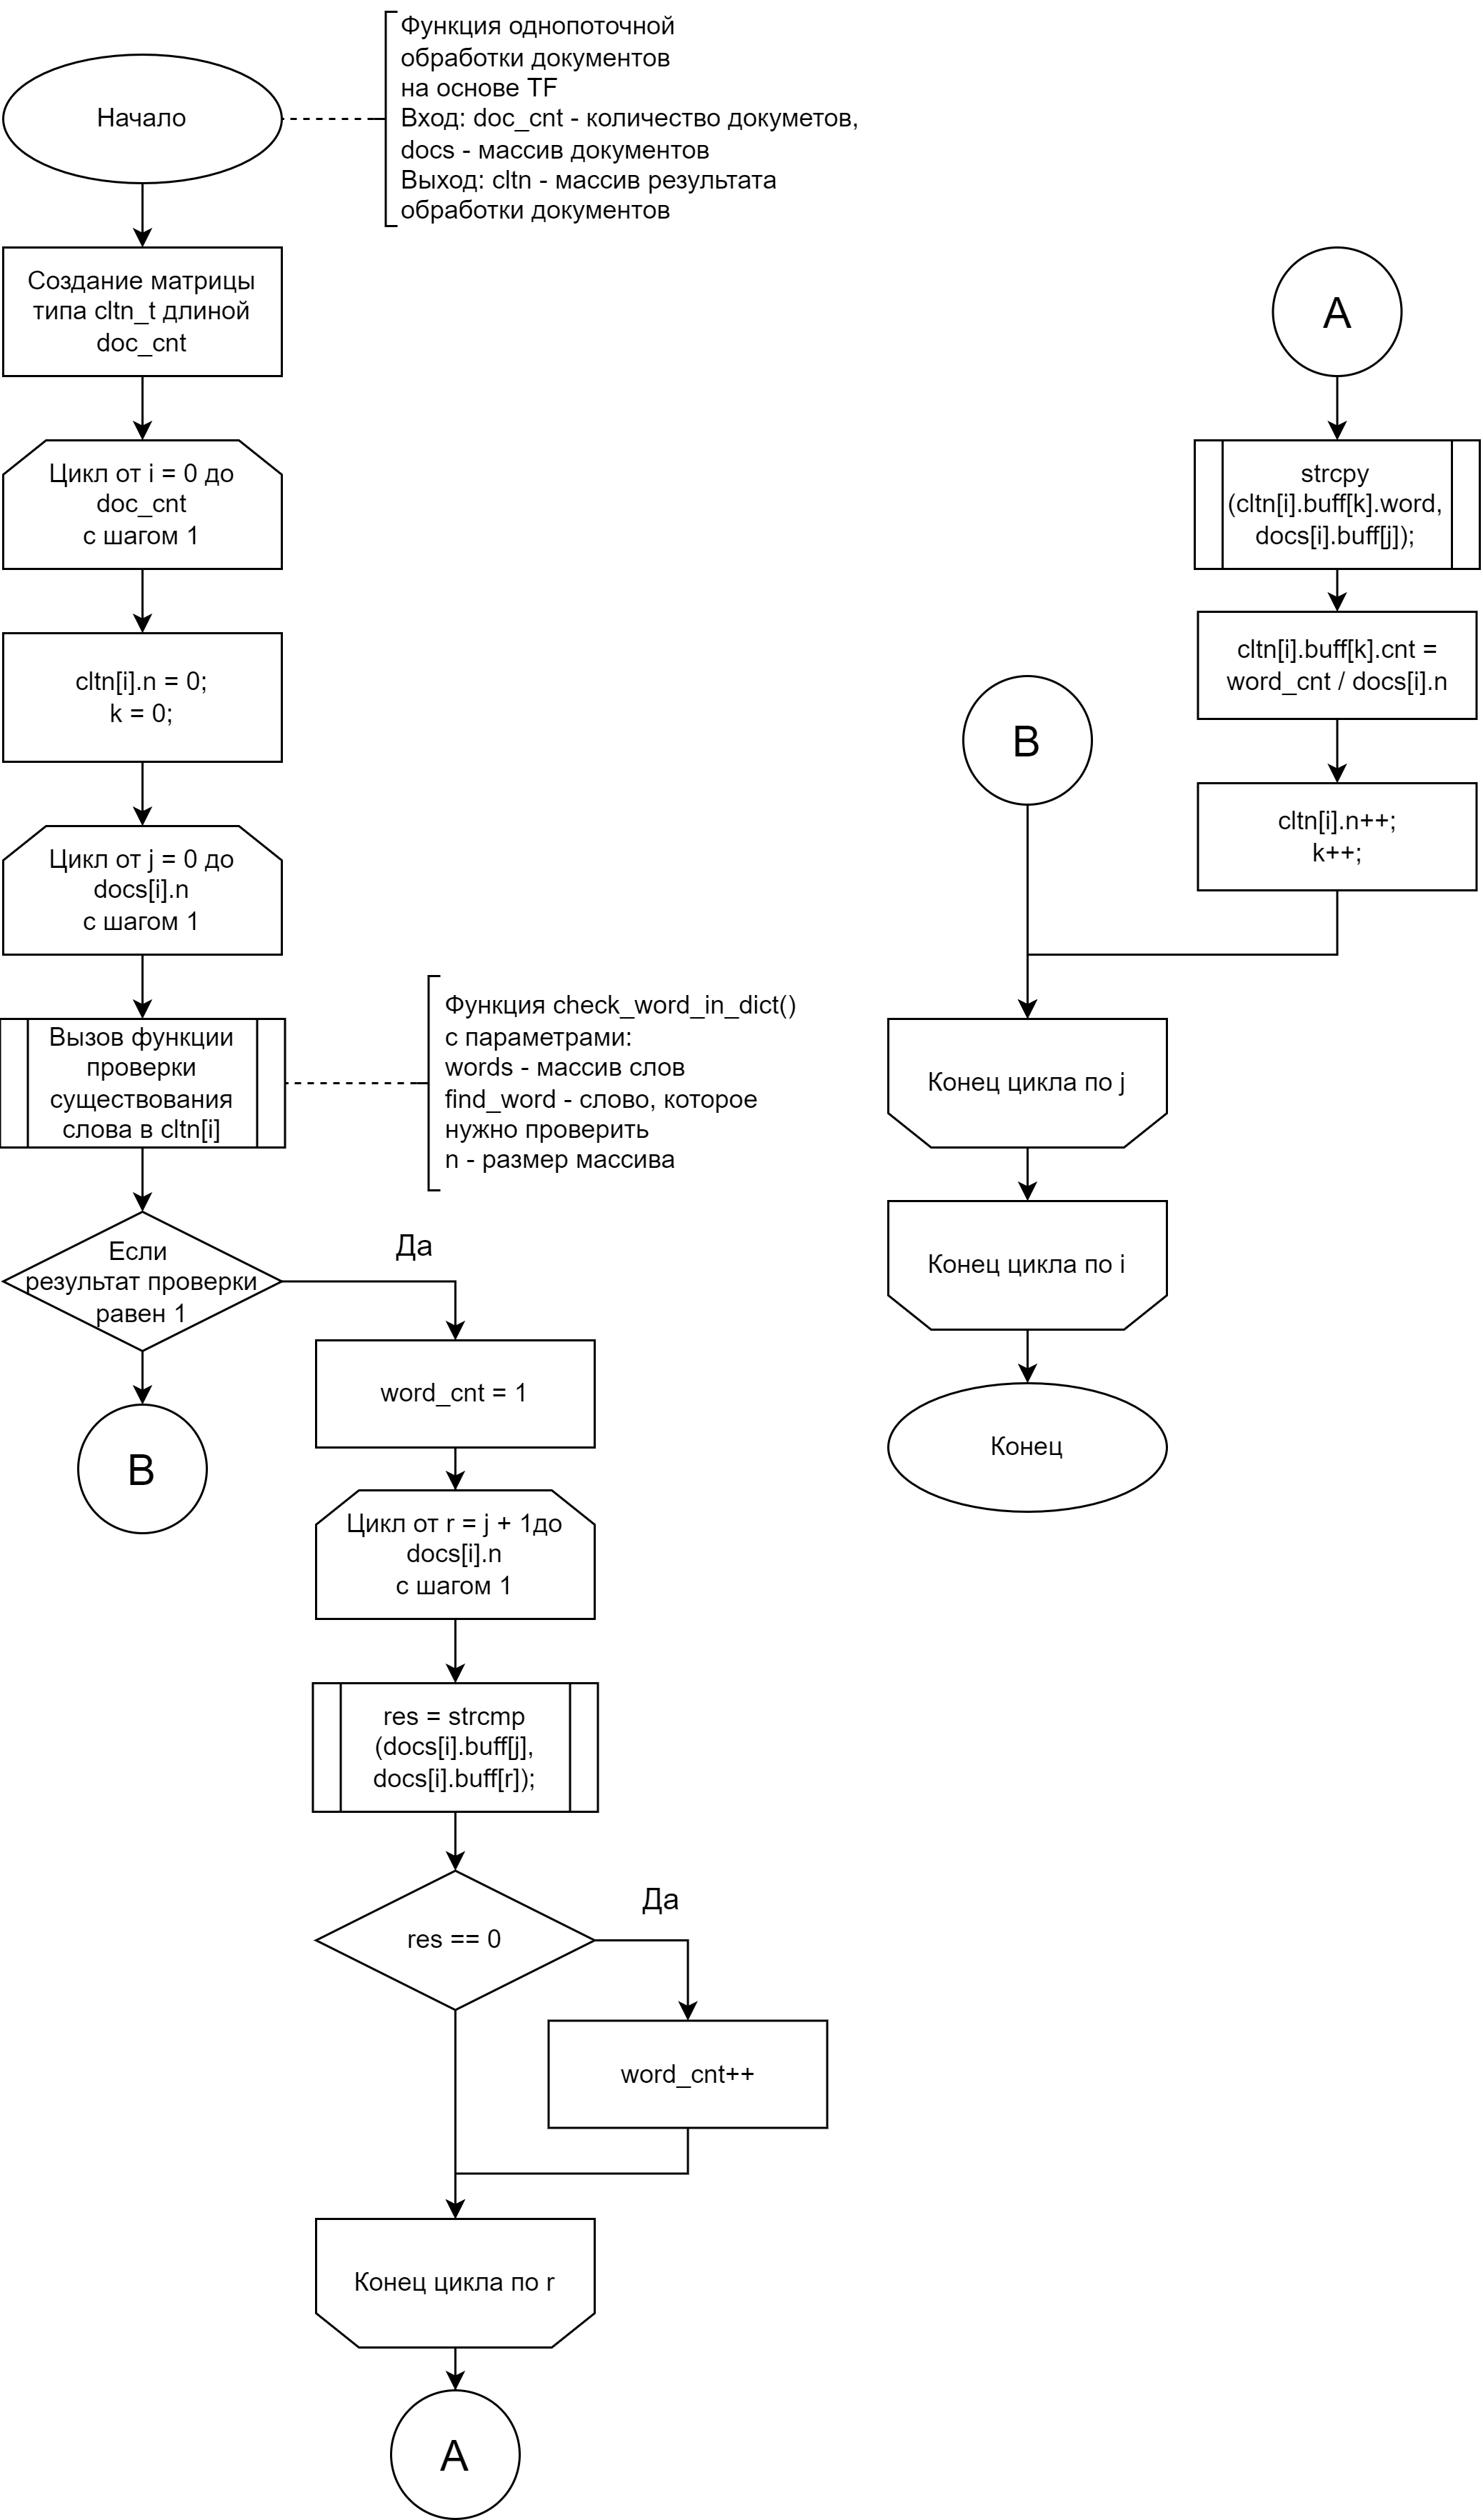
\includegraphics[width=0.85\textwidth]{img/tf_alg.png}
	\caption{Схема однопоточного алгоритма расчета термовой частота для всех термов из выборки документов}
	\label{fig:tf}
\end{figure}

\clearpage

\begin{figure}[h]
	\centering
	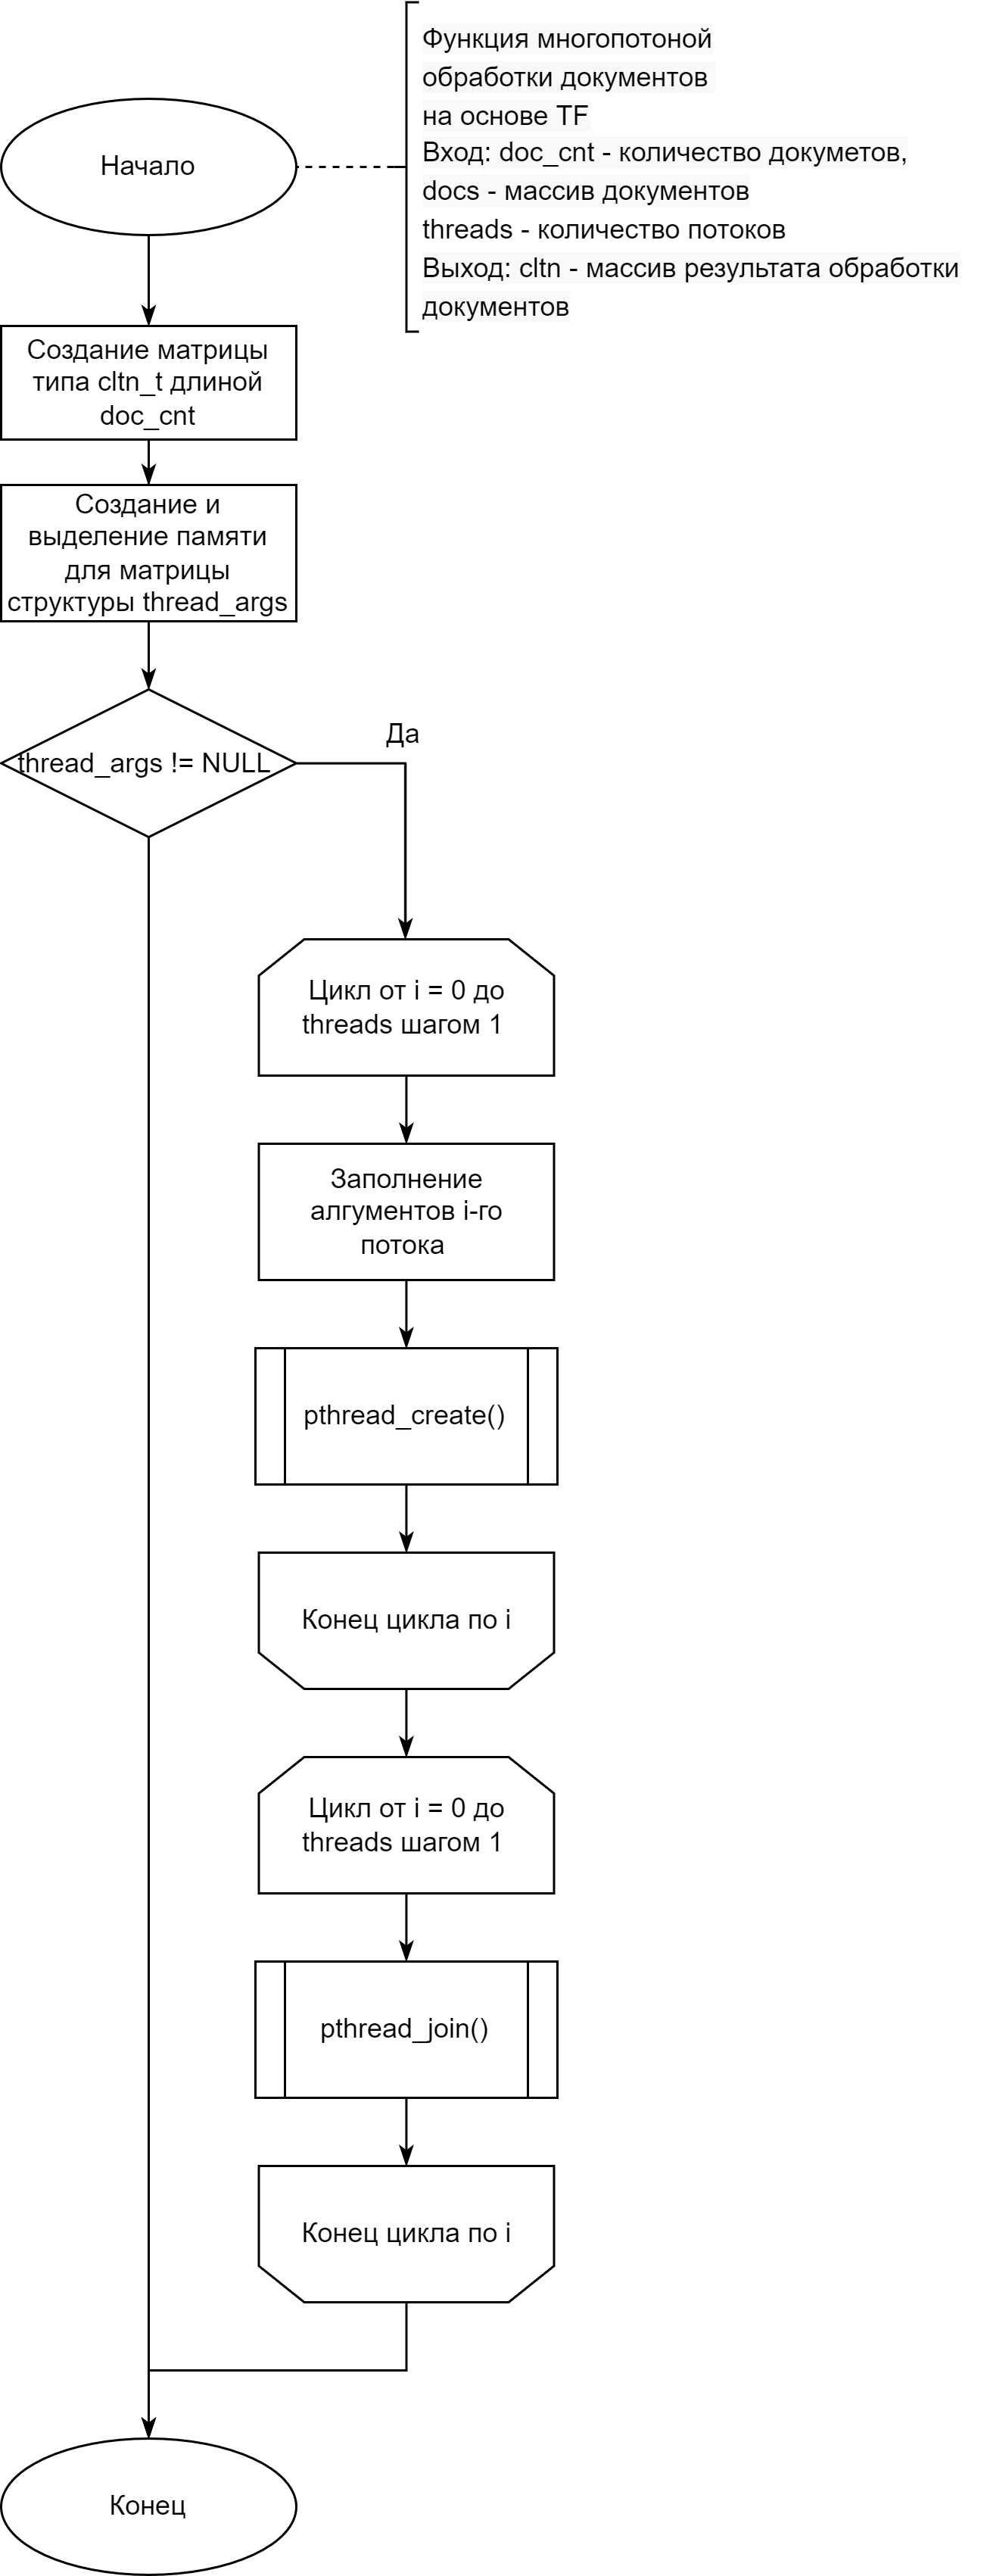
\includegraphics[height=0.85\textheight]{img/parallel.png}
	\caption{Схема алгоритма работы основного потока, запускающего вспомогательные потоки}
	\label{fig:parallel}
\end{figure}

\clearpage

\begin{figure}[h]
	\centering
	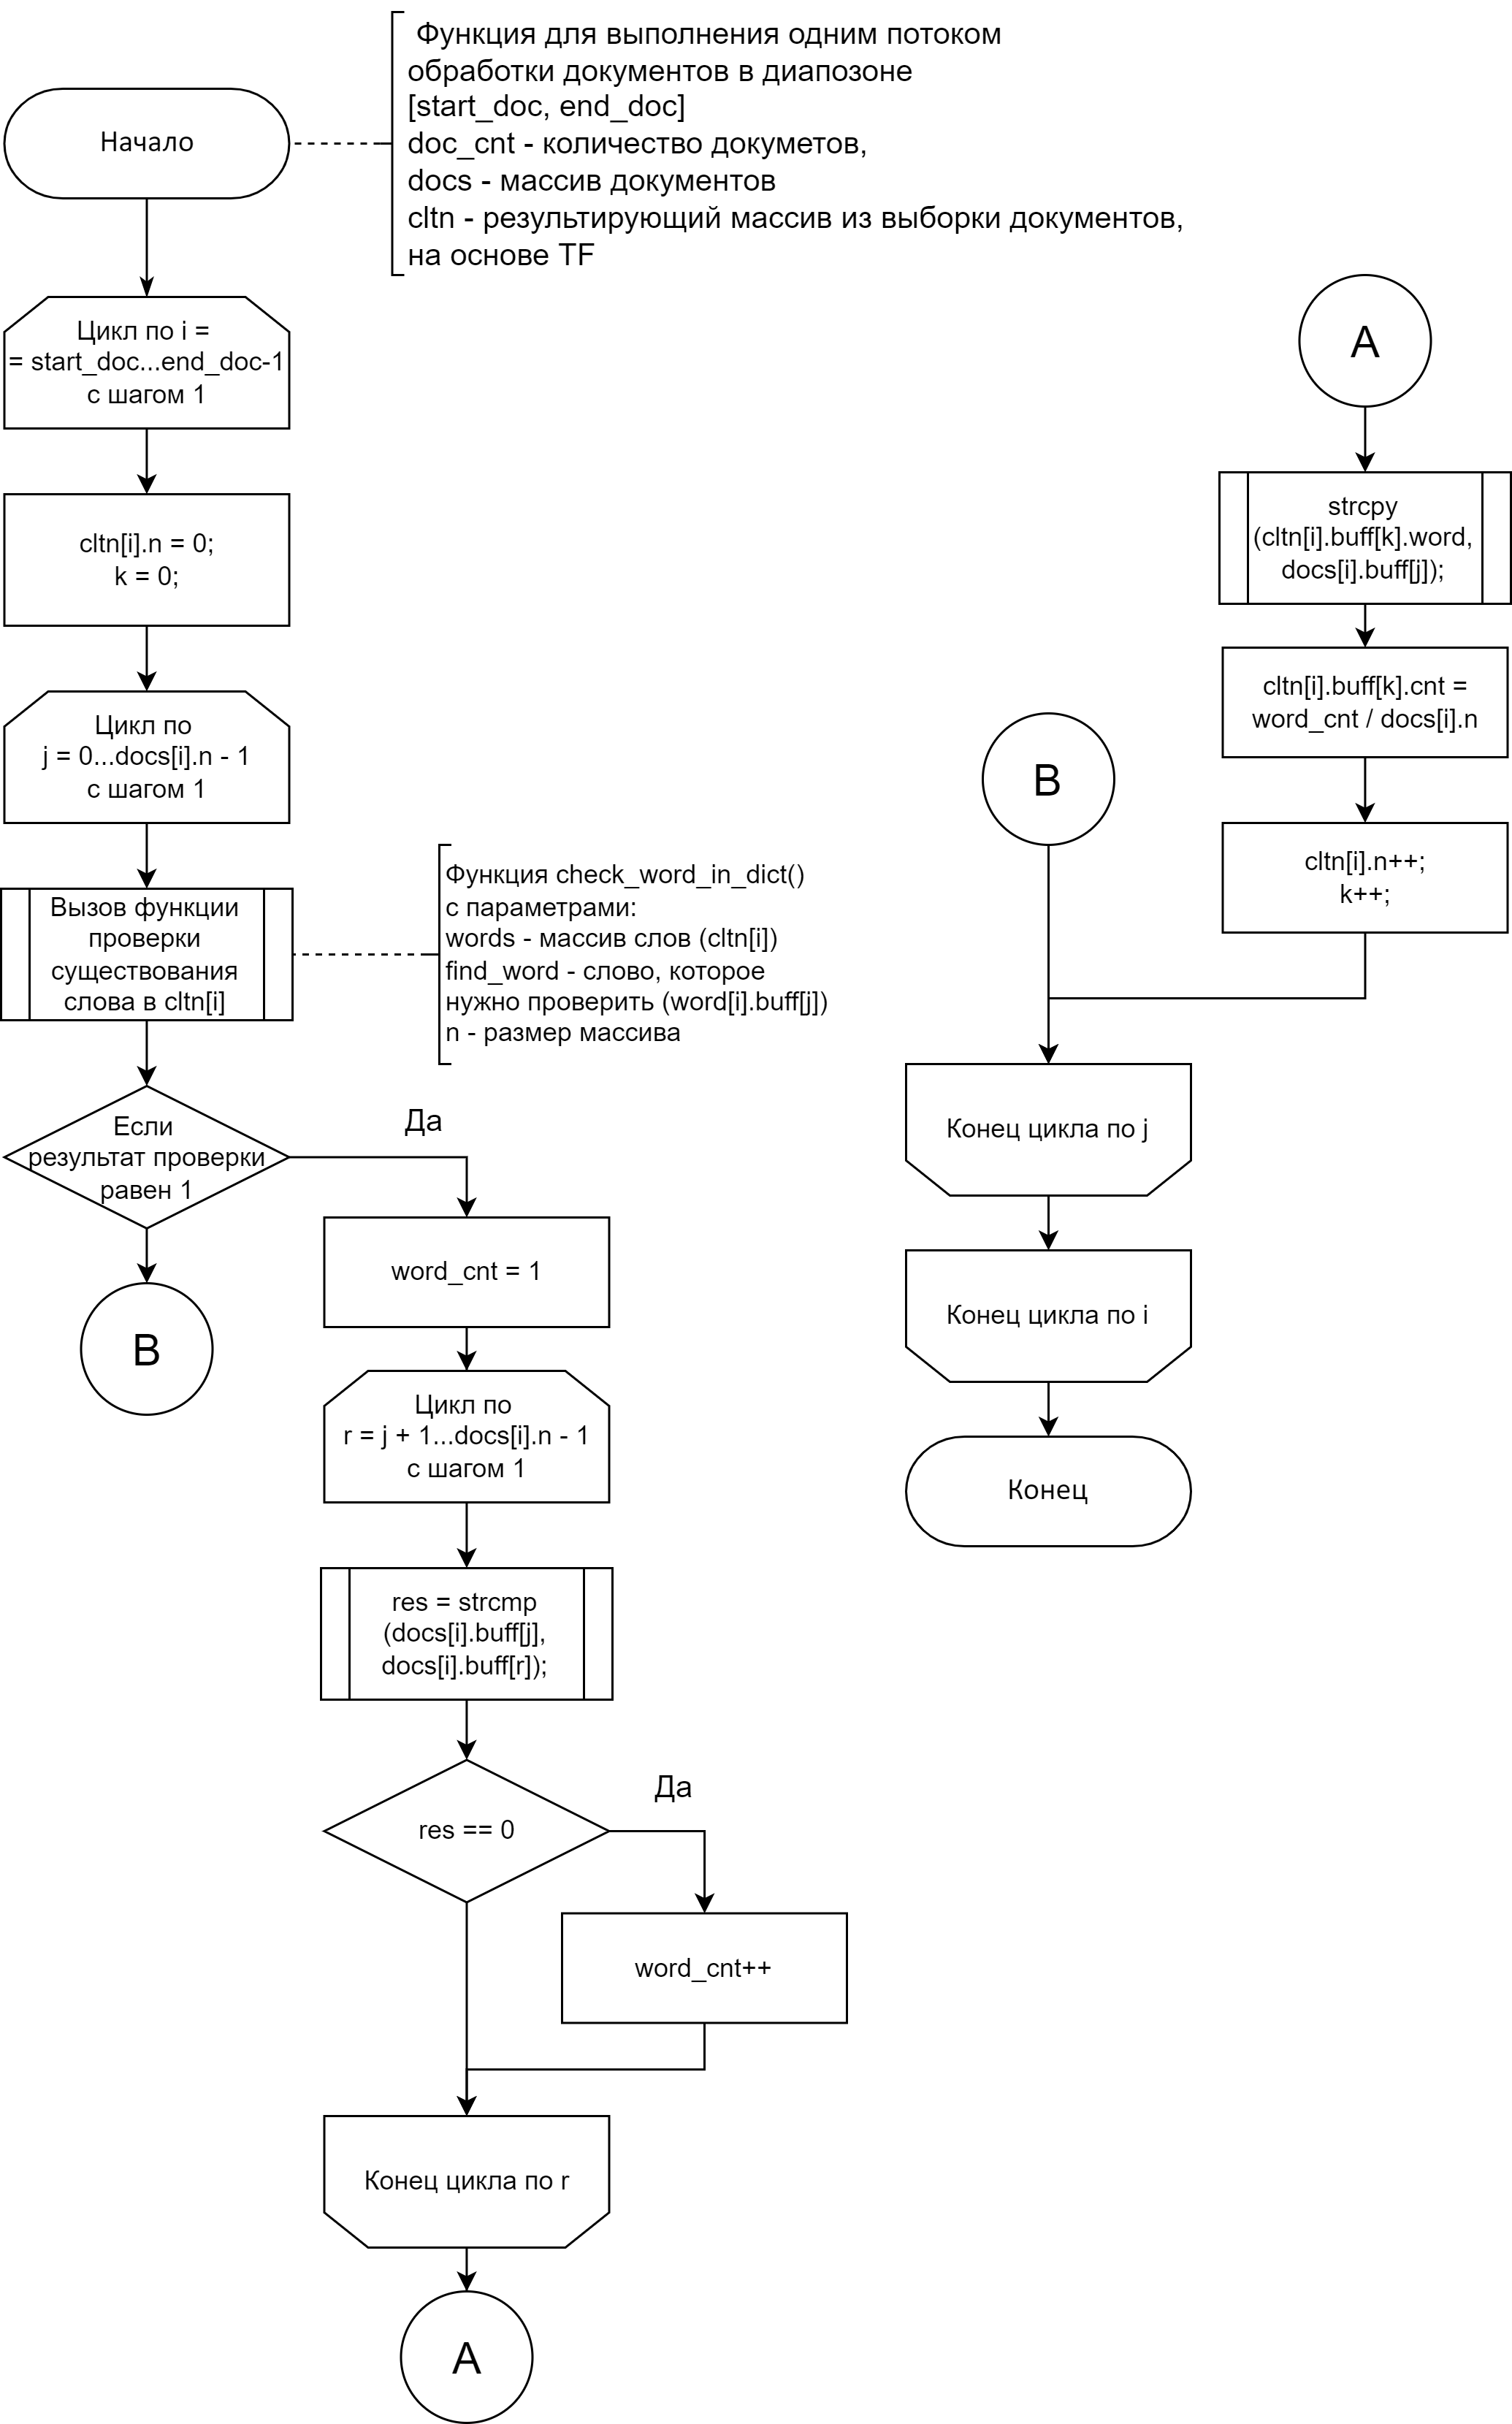
\includegraphics[height=0.85\textheight]{img/thread_work.png}
	\caption{Схема алгоритма расчета термовой частота для всех термов из выборки документов для вспомогательного потока}
	\label{fig:thread_work}
\end{figure}

\clearpage

\begin{figure}[h]
	\centering
	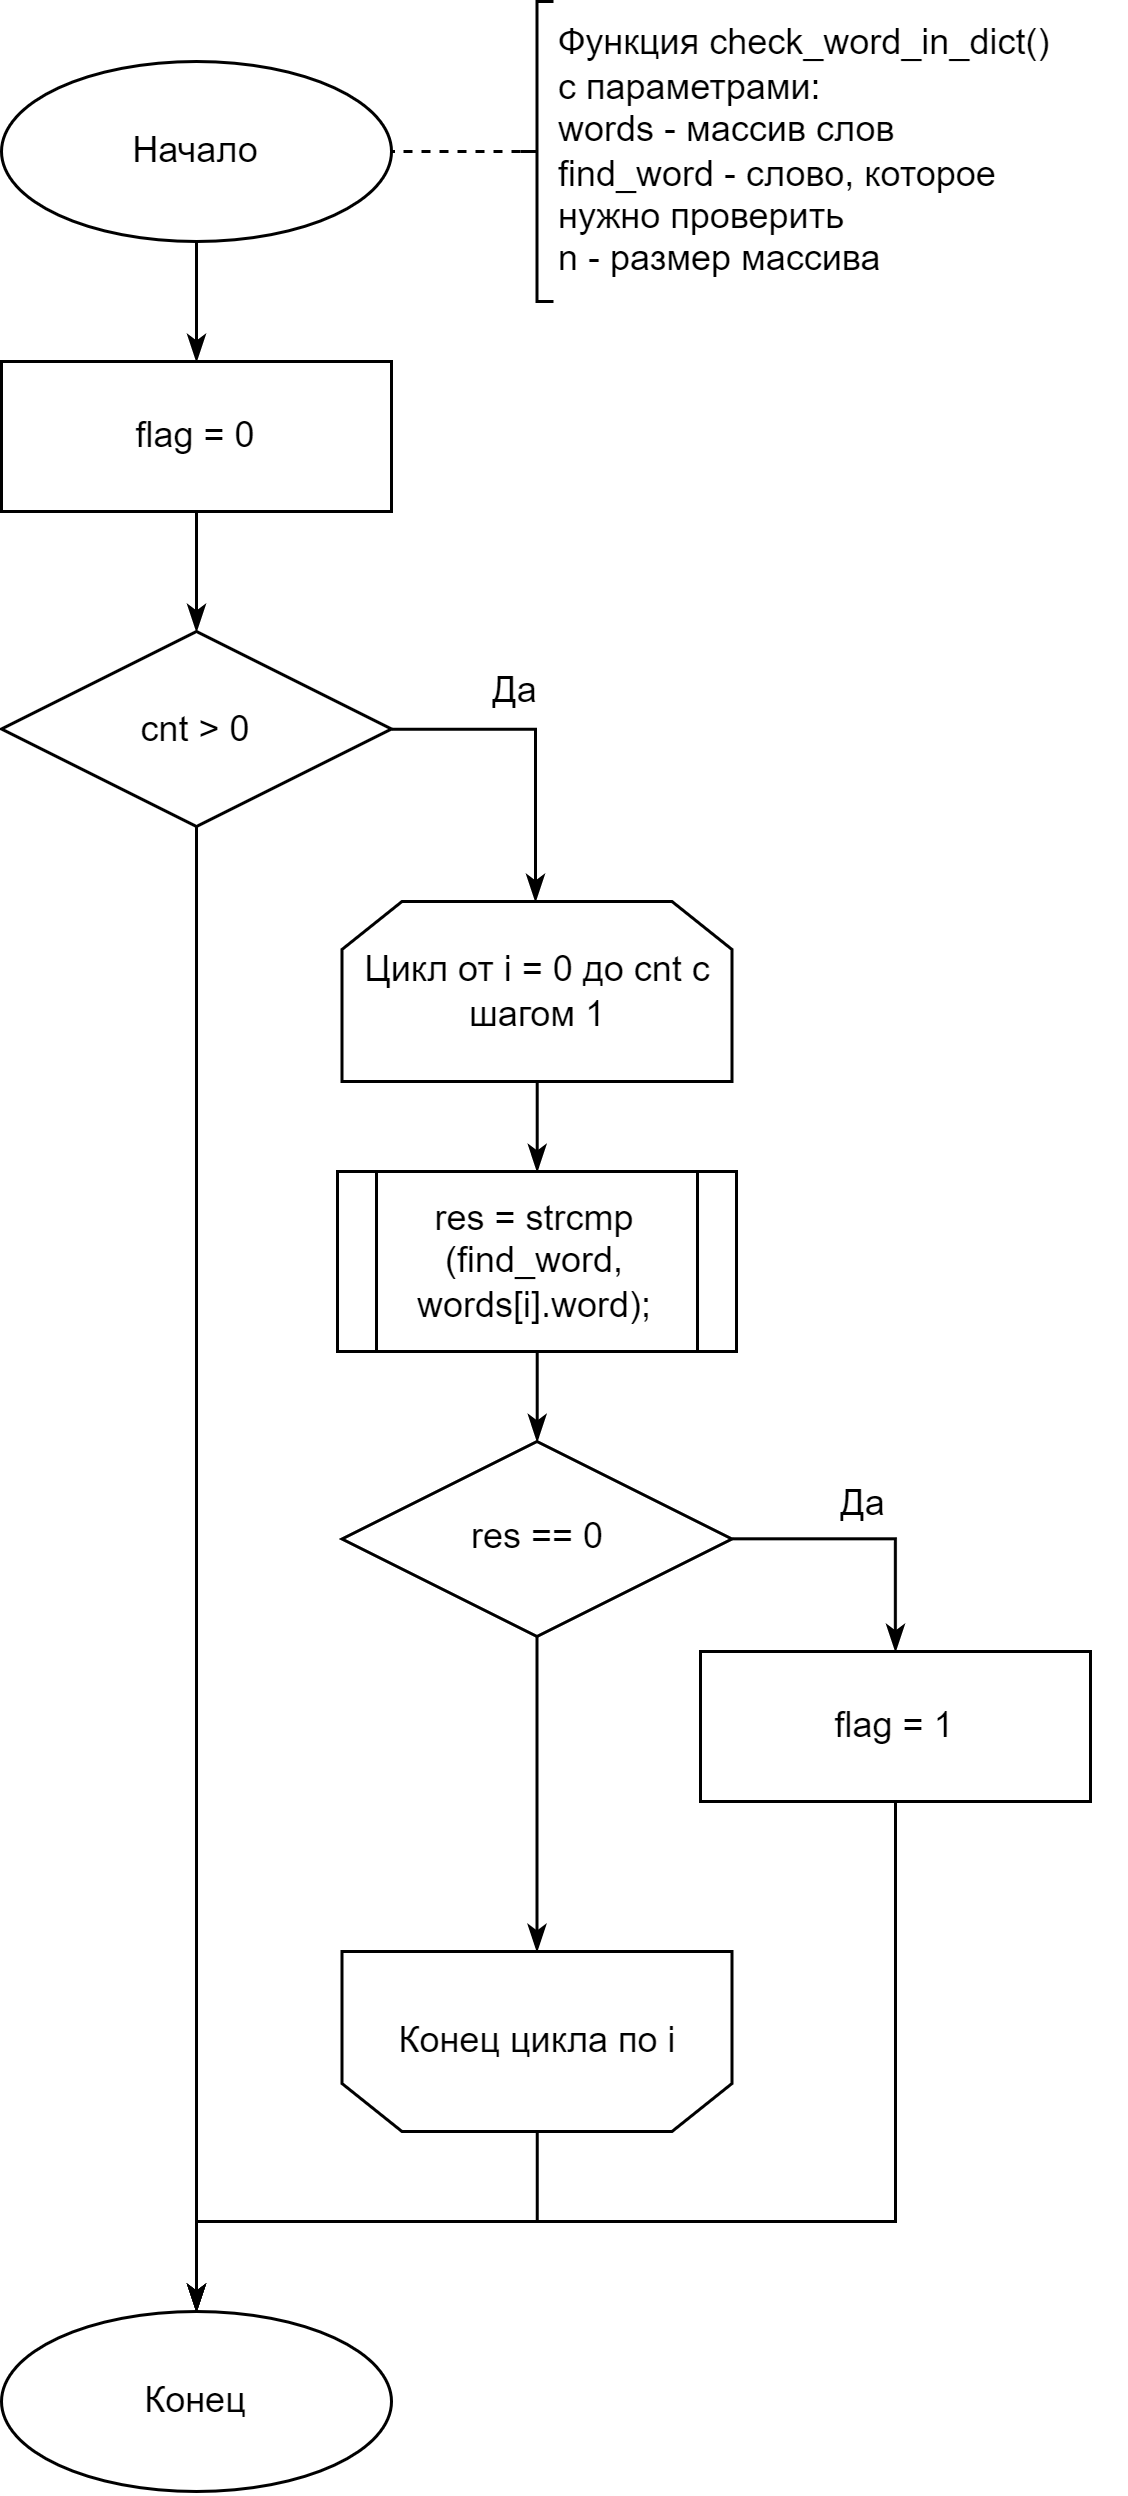
\includegraphics[height=0.7\textheight]{img/check_word.png}
	\caption{Схема алгоритма проверки существования слова в массиве}
	\label{fig:check}
\end{figure}

\section*{Вывод}

В данном разделе разработаны схемы реализаций рассматриваемого алгоритма